\beginsong{Gospodar}[mel={Rudi Rogoll, 1984}, txt={Theodor Kramer, 1984}, bo={172}, pfiii={64}]

\markboth{\songtitle}{\songtitle}

\beginverse
\endverse

\centering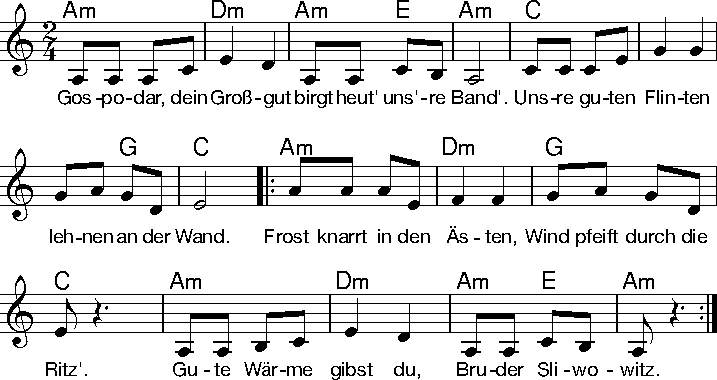
\includegraphics[width=1\textwidth]{Noten/Lied047.pdf}	

\beginverse
\[Am]Treiben wir die \[Dm]Fremden \[Am]über's \[E]Jahr erst \[Am]aus.
\[C]Gospodar, wer glaubst du, \[G]bleibt im Herrschafts\[C]haus?
\lrep \[Am]Werd' ich knechtisch \[Dm]aufsteh'n, \[G7]wo ich mächtig \[C]sitz'?
\[Am]Sind nicht solche \[Dm]Tölpel, \[Am]Bruder \[E]Sliwo\[Am]witz. \rrep
\endverse

\beginverse
^Haben unser ^Herzblut ^nichts für ^nichts ver^tan.
^Alles für die Seinen ^will der Parti^san:
\lrep ^Mutterschaf und ^Lämmer, ^Gänse, Geiß und ^Kitz,
^Kürbis und Me^lonen, ^Mais und ^Sliwo^witz. \rrep
\endverse

\beginverse
^Sind die wilden ^Schweine ^aus dem ^Land ver^jagt,
^die verkohlten Hütten ^aufgebaut und ^ragt
\lrep ^blank im Dorf der ^Maibaum, ^Flattern und Ge^fitz;
^oh, wie wird das ^schön sein, ^Bruder ^Sliwo^witz. \rrep
\endverse

\endsong

\beginscripture{}
Gospodar kommt aus dem slawischen und bedeutet Gaststätte.

Sliwowitz ist ein in Osteuropa verbreiteter Pflaumenbranntwein.
\endscripture

\begin{intersong}

\end{intersong}